\section{Sparse Identification of Nonlinear Functions Framework}
Core loss spans several orders of magnitude, so the loss function selection is important. An absolute-error objective is dominated by the high-excitation points, so a composite relative objective is used instead:
\begin{equation}
    \mathcal{L}(\boldsymbol{\xi}) =
    \underbrace{\frac{w_1}{N}\sum_{i=1}^{N}\big(\ln\hat{P}_{v,i}-\ln\bar{P}_{v,i}\big)^{2}}_{\text{logarithmic term}}
    + \underbrace{\frac{w_2}{N}\sum_{i=1}^{N}\left|\frac{\hat{P}_{v,i}-\bar{P}_{v,i}}{\bar{P}_{v,i}}\right|}_{\text{MAPE term}}
    \label{eq:objective}
\end{equation}
where $\boldsymbol{\hat{P}_v}=\boldsymbol{\Theta}(f,B) \cdot \boldsymbol{\hat{\xi}}$ is the estimated core loss and $w_1$, $w_2$ are the weights of the two contributions. The logarithmic term of mean squared error shapes the fit over the full dynamic range, while the Mean Absolute Percentage Error (MAPE) term directly targets the reported metric.

% where $\boldsymbol{\hat{P}}_v=\boldsymbol{\Theta}(f,B) \cdot \boldsymbol{\hat{\xi}}$ is the estimated core loss and $w_1$, $w_2$ weight the two contributions. The two terms are complementary rather than redundant. The logarithmic term measures the residual as a ratio, so every decade of the operating range contributes equally, and being smooth and quadratic in $\ln \hat{P}_v$ it supplies a well-conditioned gradient far from the solution. The Mean Absolute Percentage Error (MAPE) term directly targets the metric by which core loss models are reported and compared, but its gradient is piecewise constant and provides no curvature information. Combining them lets the logarithmic term drive the early descent while the MAPE term shapes the final accuracy on the reported metric.


The problem is then solved by a common AdamW optimizer with a learning rate $\eta$ and a small constant $\epsilon$ for safety. At the $j$-th epoch, the AdamW optimizer updates the coefficients by:

% with a learning rate $\eta$ and a regularizer $\epsilon$:
\begin{equation}
    \boldsymbol{\xi}^{(j+1)} = \max\!\left[
    \boldsymbol{\xi}^{(j)} - \eta \left( 
    \frac{\hat{\boldsymbol{m}}^{(j)}}{\sqrt{\hat{\boldsymbol{v}}^{(j)}}+\epsilon}
    + \gamma\,\boldsymbol{\xi}^{(j)} \right),\;\mathbf{0}\right]
    \label{eq:adamw}
\end{equation}
where $\boldsymbol{\hat{m}}^{(j)}$ and $\boldsymbol{\hat{v}}^{(j)}$ are bias-corrected momenta from the AdamW algorithm, $\gamma$ is the weight decay rate, and the projection enforces non-negativity. During the updates, $\gamma$ pulls $\xi$ of candidates containing minor contribution toward zero and is pinned at zero by a binary mask if it is below the pruning threshold $\lambda_{\mathrm{max}}$. The pruning mechanism leads to refined sparse $\boldsymbol{\xi}$ that represent a simple explicit core loss equation. Note that $\boldsymbol{\xi}$ are constrained to be non-negative, which enforces that every retained term contributes positively to the total loss. With a refined sparse $\boldsymbol{\xi}$, the core loss equation can thus be identified with simple symbolic expressions, as shown in Fig.~\ref{fig:framework}. The comprehensive steps will be shown in full paper.


\begin{figure}[t] 
    \centering
    \vspace{-5pt}
    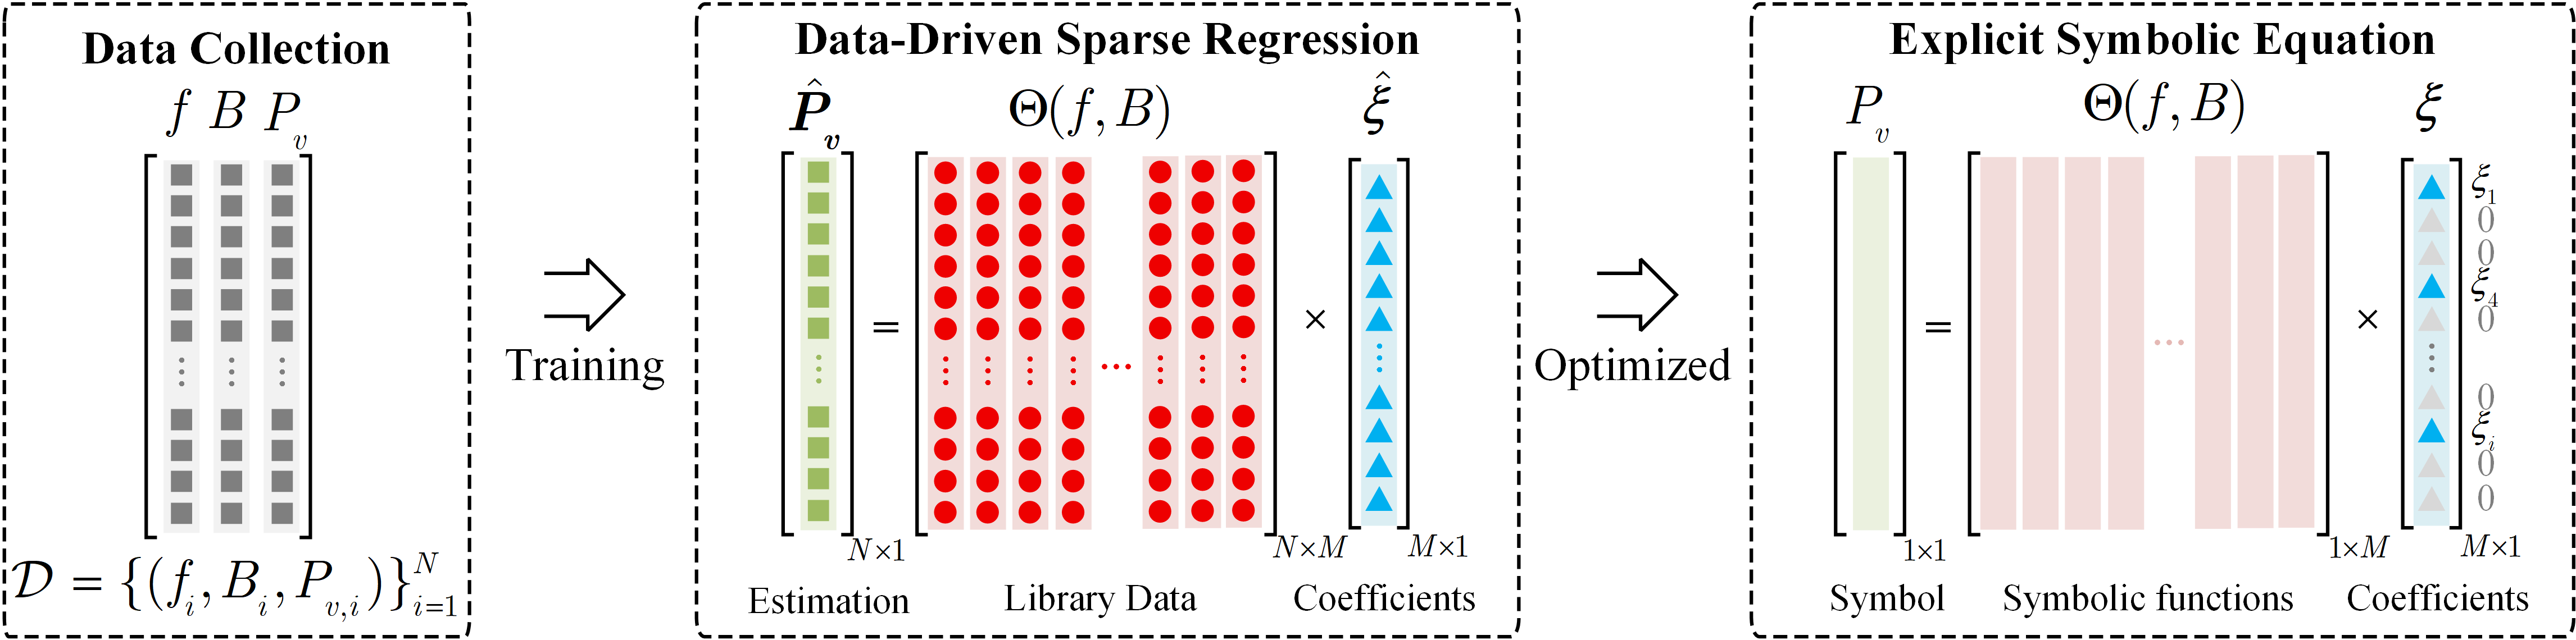
\includegraphics[width=0.95\textwidth]{Figure1.png} 
    \vspace{-5pt}
    \caption{The proposed SINF framework including data-driven sparse regression and function discovery.}
    \label{fig:framework}
\end{figure}

% Support selection is completed by a ramped hard threshold applied to the
% normalized coefficients. Over the last $(1-\rho)$ fraction of the discovery
% phase, the threshold grows linearly,
% \begin{equation}
%     \lambda^{(j)} = \lambda_{\max}\,
%     \min\!\left(\frac{j-\rho J}{(1-\rho)J},\,1\right),
%     \label{eq:ramp}
% \end{equation}
% and every $\Delta_p$ epochs the terms satisfying $\xi_k<\lambda^{(j)}$ are
% removed by a binary mask. The gradual ramp lets the surviving terms absorb the
% contribution of each removal before the next one, and the optimizer state is
% reset after every removal so that the adaptive moments describe the reduced
% landscape rather than the previous one.




